%Die Angabe des schlauen Spruchs auf diesem Wege funtioniert nur,
%wenn keine Änderung des Kapitels mittels den in preambel/chapterheads.tex
%vorgeschlagenen Möglichkeiten durchgeführt wurde.
\chapter{Machine Learning}
\label{chap:chapter3}
%\vspace{-3cm}
%\vspace{2cm}
An \emph{algorithm} is set of instructions used to convert input values to output, based on certain rules. Consider an example where we need to find all even numbers from dataset. Here, we can set up a \emph{rule} that if number is completely divisible by two then it should be included in the output dataset, otherwise not. Naturally, as there can be more than one way to solve a problem, there can be more than one algorithm to solve it. However there are certain examples where formation of set of rule is practically infeasible. For example, consider handwriting recognition software used to scan handwritten forms. Figure illustrates problem at hand, where a simple character can be written in a number of ways. It is interesting to note that humans are able to read this data without trouble, but it is really difficult express a certain rules which will result in accurate recognition with help of an algorithm. Machine learning is employed in such cases. Specifically \emph{Machine Learning} (ML) is programming computers to optimize a performance criterion (e.g. character recognition) using example data or past experience \cite{Alpaydin2004}. 

\begin{figure}[h]
  \begin{center}
    \captionsetup{justification=centering}
    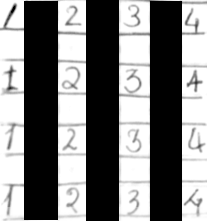
\includegraphics[scale=0.5]{figures/charrec.png}
    \caption{Example of Machine Learning: Character recognition}
    \label{fig:charrec}
  \end{center}
\end{figure}

The "example data" with its \emph{label} is collectively called as \emph{training data}, and it is used to teach machine learning how the character with given label looks like, so that ML can recognize when it encounters similar data in future. Machine learning can be applied in wide range of applications where it is not possible to express expertise but a large amount of sample data is available. Typical applications of machine learning include computer vision, pattern recognition, spam filtering, search result optimization etc. 

\section{Basics of Machine Learning}
\label{sec:c3basics}

\subsection{Types of learning algorithms}
Based on application, ML algorithms can be can be classifed in two major catagories \emph{viz.} supervised learning and unsupervised learning. 

\emph{Supervised learning} algorithms are used when labels of the data to be are known. A spam filter is a good example where supervised learning can be used for \emph{classification}. Here we know an email received is either "spam" or "not-spam", these catagories can be used as labels for the sample population and learning algorithm can classify within these two type.  One more application of supervised learning is to predict a numerical value in \emph{regression}. Consider a problem to prdict value of a used property, the input parameters in this case are initial value, year of constuction, size of property, locality and so on, whereas output is current resale value. one can construct a training dataset of known resale values and repective values of input parameters and train leaning algorithm to predict other inputs. To generalize, aim in supervised learning is to learn mapping from input to output whose correct vales are provided by supervisor \cite{Alpaydin2004}.

\emph{Unsupervised learning} or \emph{clustering} is used in classification problems where the labels for the data are not known. An example of such problem is document clustering \cite{Alpaydin2004}. In this problem aim is to cluster news reports which belong to same catagory like sport, science, art and so on. The number of such catagories is not clear, and the machine learning application in such case needs to cluster articles based on some common words, and provide the supervisor data, which he may use to label clustered groups.

\subsection{Features and Feature Selection}
A \emph{feature} $(\chi_i)$ is a result of measurement made on a unit input data. In general, a set of features $(\boldsymbol{\chi}^t)$ is needed to characterize a unit input data,
\[ \boldsymbol{\chi}^t = 
\left[ \begin{array}{c}
\chi_1\\
\chi_2 \\
.\\
.\\
\chi_n \end{array} \right]\]  

and its label $r$ denotes its type
\[ r = \left\{ \begin{array}{ll}
         0 & \mbox{if $\chi$ belongs to class 0};\\
         1 & \mbox{if $\chi$ belongs to class 1 and so on..}\end{array} \right. \] 


\subsection{Sample population}

\section{Machine Learning Algorithms for Classification}
\label{sec:c3mlclassification}

\subsection{Bayesian networks}

\subsection{Descision Trees}

\subsection{Multilayered Perceptrons}

\subsection{Support Vector Machines}

\section{Criterion To Choose Suitable ML Algorithm}
\label{sec:c3mlselection}
